% !TEX root = main.tex
\chapter{Real time decoder}
\label{cha:decoder}

% The \ac{HTK} decoders are not real-time decoders\cite{yao2010practical}. 
\todo{Ten development vyhodit. Ty uz nemas cas na zadny vyvoj. Radeji dej do evaluation, ze rozeberes nejenom presnost 
ale i rychlosty dekoderu, a rohodnes ktery dekoder z Kaldi je vhodny a jake nastaveni potrebuje pro RT performance.}

\todo{We used OpenJulius for decoding lattices and normal outputs -- describe again the problems}
\todo{Mention the socket! API of OpenJulius}
\todo{dat tam analyza -> future improvements}
\todo{udelat real time experiment }
\todo{srovnani Julius prohledavani   pulka stranky}
\section{Online decoder original architecture} 
\label{sec:kaldi_decoder_architecture}
This section describes the architecture online decoder developed by Kaldi team.
The online decoder was used as starting point for building \ac{FST} real time decoder for our dialog system.

\begin{figure}[!ph]
    \begin{center}
        % Graphic for TeX using PGF
% Title: /home/ondra/Diagram1.dia
% Creator: Dia v0.97.2
% CreationDate: Thu Aug  1 08:02:11 2013
% For: ondra
% \usepackage{tikz}
% The following commands are not supported in PSTricks at present
% We define them conditionally, so when they are implemented,
% this pgf file will use them.
\ifx\du\undefined
  \newlength{\du}
\fi
\setlength{\du}{15\unitlength}
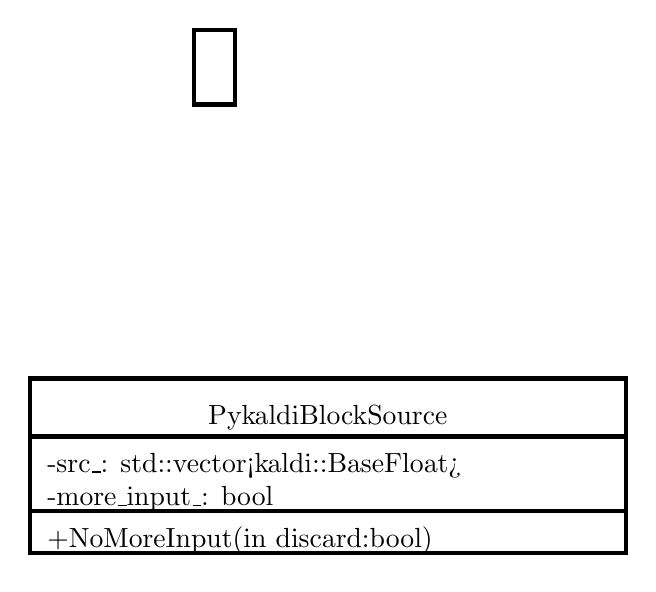
\begin{tikzpicture}
\pgftransformxscale{1.000000}
\pgftransformyscale{-1.000000}
\definecolor{dialinecolor}{rgb}{0.000000, 0.000000, 0.000000}
\pgfsetstrokecolor{dialinecolor}
\definecolor{dialinecolor}{rgb}{1.000000, 1.000000, 1.000000}
\pgfsetfillcolor{dialinecolor}
\pgfsetlinewidth{0.100000\du}
\pgfsetdash{}{0pt}
\definecolor{dialinecolor}{rgb}{1.000000, 1.000000, 1.000000}
\pgfsetfillcolor{dialinecolor}
\fill (13.250000\du,6.900000\du)--(13.250000\du,8.700000\du)--(14.250000\du,8.700000\du)--(14.250000\du,6.900000\du)--cycle;
\definecolor{dialinecolor}{rgb}{0.000000, 0.000000, 0.000000}
\pgfsetstrokecolor{dialinecolor}
\draw (13.250000\du,6.900000\du)--(13.250000\du,8.700000\du)--(14.250000\du,8.700000\du)--(14.250000\du,6.900000\du)--cycle;
% setfont left to latex
\definecolor{dialinecolor}{rgb}{0.000000, 0.000000, 0.000000}
\pgfsetstrokecolor{dialinecolor}
\node at (13.750000\du,7.995000\du){};
% setfont left to latex
\pgfsetlinewidth{0.050000\du}
\definecolor{dialinecolor}{rgb}{0.000000, 0.000000, 0.000000}
\pgfsetstrokecolor{dialinecolor}
\draw (13.750000\du,8.147500\du)--(13.750000\du,8.147500\du);
\pgfsetlinewidth{0.100000\du}
\pgfsetdash{}{0pt}
\definecolor{dialinecolor}{rgb}{1.000000, 1.000000, 1.000000}
\pgfsetfillcolor{dialinecolor}
\fill (9.300000\du,15.300000\du)--(9.300000\du,16.700000\du)--(23.660000\du,16.700000\du)--(23.660000\du,15.300000\du)--cycle;
\definecolor{dialinecolor}{rgb}{0.000000, 0.000000, 0.000000}
\pgfsetstrokecolor{dialinecolor}
\draw (9.300000\du,15.300000\du)--(9.300000\du,16.700000\du)--(23.660000\du,16.700000\du)--(23.660000\du,15.300000\du)--cycle;
% setfont left to latex
\definecolor{dialinecolor}{rgb}{0.000000, 0.000000, 0.000000}
\pgfsetstrokecolor{dialinecolor}
\node at (16.480000\du,16.250000\du){PykaldiBlockSource};
\definecolor{dialinecolor}{rgb}{1.000000, 1.000000, 1.000000}
\pgfsetfillcolor{dialinecolor}
\fill (9.300000\du,16.700000\du)--(9.300000\du,18.500000\du)--(23.660000\du,18.500000\du)--(23.660000\du,16.700000\du)--cycle;
\definecolor{dialinecolor}{rgb}{0.000000, 0.000000, 0.000000}
\pgfsetstrokecolor{dialinecolor}
\draw (9.300000\du,16.700000\du)--(9.300000\du,18.500000\du)--(23.660000\du,18.500000\du)--(23.660000\du,16.700000\du)--cycle;
% setfont left to latex
\definecolor{dialinecolor}{rgb}{0.000000, 0.000000, 0.000000}
\pgfsetstrokecolor{dialinecolor}
\node[anchor=west] at (9.450000\du,17.400000\du){-src\_: std::vector<kaldi::BaseFloat>};
% setfont left to latex
\definecolor{dialinecolor}{rgb}{0.000000, 0.000000, 0.000000}
\pgfsetstrokecolor{dialinecolor}
\node[anchor=west] at (9.450000\du,18.200000\du){-more\_input\_: bool};
\definecolor{dialinecolor}{rgb}{1.000000, 1.000000, 1.000000}
\pgfsetfillcolor{dialinecolor}
\fill (9.300000\du,18.500000\du)--(9.300000\du,19.500000\du)--(23.660000\du,19.500000\du)--(23.660000\du,18.500000\du)--cycle;
\definecolor{dialinecolor}{rgb}{0.000000, 0.000000, 0.000000}
\pgfsetstrokecolor{dialinecolor}
\draw (9.300000\du,18.500000\du)--(9.300000\du,19.500000\du)--(23.660000\du,19.500000\du)--(23.660000\du,18.500000\du)--cycle;
% setfont left to latex
\definecolor{dialinecolor}{rgb}{0.000000, 0.000000, 0.000000}
\pgfsetstrokecolor{dialinecolor}
\node[anchor=west] at (9.450000\du,19.200000\du){+NoMoreInput(in discard:bool)};
\end{tikzpicture}

    \caption{Aggregation of classes for serial input processing}
    \label{fig:classes} 
    \end{center}
\end{figure}

\todo{Describe architecture}
% section kaldi_decoder_architecture (end)

\section{Improving online decoder} 
\label{sec:improve}
We will present how we overcome the limitations of Kaldi online decoder.

% section online_decoder_improvements (end)


\section[Comparison of real time decoders]{Comparison of real time decoders in Alex dialog system} 
\label{sec:comparison_of_real_time_decoders_in_alex_dialog_system}
Further, in this section we will briefly compare the main qualities of used decoders.
Namely, we will compare: 
\begin{itemize}
    \item Kaldi online decoder - Acoustic models were trained by training scripts for Kaldi described at~\ref{cha:models}.
    \item OpenJulius - OpenJulius uses in our setup acoustic models trained by \ac{HTK}. 
    \item HDecode - HDecode is \ac{HTK} decoder and it decodes from acoustic models trained by \ac{HTK}.
\end{itemize}


% section comparison_of_real_time_decoders_in_alex_dialog_system (end)
% chapter real_time_decoder (end)
